\documentclass{standalone}
%-----------------------------------------------------------------------------%
%%% Color %%%
\usepackage{xcolor}
\definecolor{myred}{RGB}{229,0,0}
\definecolor{myblue}{RGB}{0,98,144}
\definecolor{myyellow}{RGB}{246,182,50}
\newcommand{\red}[1]{\textcolor{myred}{#1}}
\newcommand{\blue}[1]{\textcolor{myblue}{#1}}
\newcommand{\yellow}[1]{\textcolor{myyellow}{#1}}
%-----------------------------------------------------------------------------%
%%% TikZ %%%
\usepackage{tikz}
\usetikzlibrary{perspective}
% \usetikzlibrary{calc}
% \usetikzlibrary{positioning}
% \usetikzlibrary{patterns}
% \usetikzlibrary{fit}
% \usetikzlibrary{angles,quotes}
% \usetikzlibrary{intersections}
% \usetikzlibrary{decorations.markings}
%-----------------------------------------------------------------------------%

\begin{document}

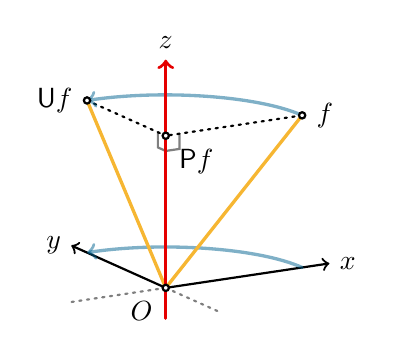
\begin{tikzpicture}[thick,line cap=round,scale=2,3d view]
	\tikzstyle{bai}=[solid,circle,draw,inner sep=.8pt,fill=white];
	\tikzstyle{hei}=[solid,circle,draw,inner sep=.8pt,fill];
	%% Axes
	\draw[->] (0,0,0) -- (1.2,0,0) node[right]{$x$};
	\draw[->] (0,0,0) -- (0,1.2,0) node[left]{$y$};
	%% Mark Right Angles
	\draw[opacity=0.5] (0.1,0,1) -- (0.1,0,1-0.1) -- (0,0,1-0.1);
	\draw[opacity=0.5] (0,0.1,1) -- (0,0.1,1-0.1) -- (0,0,1-0.1);
	%% Dotted Axes
	\draw[dotted,opacity=0.5] (0,0,0) -- (-0.7,0,0);
	\draw[dotted,opacity=0.5] (0,0,0) -- (0,-0.7,0);
	%% Projection Path
	\draw[dotted] (1,0,1) -- (0,0,1);
	\draw[dotted] (0,1,1) -- (0,0,1);
	%% Rotation
	\draw[->,very thick,myblue,opacity=0.5] (1,0,0) arc (0:90:1);
	\draw[->,very thick,myblue,opacity=0.5] (1,0,1) arc (0:90:1);
	%% Vectors
	\draw[very thick,myyellow] (0,0,0) -- (1,0,1);
	\draw[very thick,myyellow] (0,0,0) -- (0,1,1);
	%% Invariant Subspace
	\draw[->,very thick,myred] (0,0,-0.2) -- (0,0,1.5) node[above,black]{$z$};
	%% Notes
	\node[bai,label=below left:{$O$}] at (0,0,0) {};
	\node[bai,label=below right:{$\mathsf{P}f$}] at (0,0,1) {};
	\node[bai,label=right:{$f$}] at (1,0,1) {};
	\node[bai,label=left:{$\mathsf{U}f$}] at (0,1,1) {};
\end{tikzpicture}

\end{document}
